\documentclass[a4paper]{article}

\usepackage[margin=2.05cm]{geometry}
\usepackage[T1]{fontenc}
\usepackage[utf8]{inputenc}
\usepackage{lmodern}
\usepackage{microtype}
\usepackage{amsmath,amssymb}
\usepackage{booktabs}
\usepackage{graphicx}
\usepackage{siunitx}
\usepackage{longtable}
\usepackage{array}
\usepackage{xcolor}
\usepackage{adjustbox}
\usepackage[hyphens]{url}
\usepackage{tikz}
\usetikzlibrary{arrows.meta,positioning,fit,backgrounds}
\usepackage[colorlinks=true,linkcolor=black,citecolor=black,urlcolor=blue!55!black]{hyperref}
\makeatletter
\g@addto@macro\UrlBreaks{\do\/\do\-\do\.\do\?\do\&\do\=\do\_\do\%\do\:}
\Urlmuskip=0mu plus 1mu
\makeatother
\usepackage{enumitem}
\usepackage{caption}
\captionsetup{font=small,labelfont=bf}
\setlist{itemsep=2pt,topsep=3pt,parsep=0pt}
\setlength{\intextsep}{5pt plus 2pt minus 2pt}
\setlength{\textfloatsep}{8pt plus 2pt minus 2pt}
\setlength{\abovecaptionskip}{3pt}
\setcounter{topnumber}{3}\setcounter{bottomnumber}{2}\setcounter{totalnumber}{4}
\renewcommand{\topfraction}{0.92}\renewcommand{\bottomfraction}{0.6}
\renewcommand{\textfraction}{0.06}\renewcommand{\floatpagefraction}{0.75}

\newcommand{\zindiuser}{Chispita\_1}
\newcommand{\submissionid}{KDVKc3sY (final); 1CjfM8je (earlier 5-feature blend)}
\newcommand{\coderepo}{https://github.com/Ali-Cerna-Enciso/bias-bounty-mapping-equity-submission}

\newcommand{\Ftribal}{\texttt{r\_tribal\_any}}
\newcommand{\Frural}{\texttt{rural}}
\newcommand{\Ftrans}{\texttt{g\_transport}}
\newcommand{\Froute}{\texttt{t\_route\_lowclass\_share}}
\newcommand{\Ffire}{\texttt{h\_fire\_missing\_risk}}
\newcommand{\Fpoi}{\texttt{c\_poi\_deficit\_pop}}
\newcommand{\my}{\overline{y}}
\newcommand{\R}{\mathrm{RMSE}}

\title{\vspace{-1.2cm}\textbf{Bias Bounty Mapping Equity Challenge}\\[2pt]
\large Methodology writeup for \emph{Best Documentation}}
\author{}
\date{31 October 2026}

\hypersetup{pdftitle={Bias Bounty Mapping Equity Challenge: Best Documentation},
            pdfauthor={Zindi user \zindiuser},
            pdfsubject={Best Documentation},
            pdfkeywords={coverage gap, Overture, bias, emergency access, rural health}}


\begin{document}
\maketitle
\vspace{-1.1cm}

\begin{center}
\small
\begin{tabular}{@{}ll@{}}
\toprule
Zindi username & \zindiuser \\
Leaderboard submission(s) & \submissionid \\
Code repository & \url{\coderepo} \\
Prize & Best Documentation \\
\bottomrule
\end{tabular}
\end{center}

\begin{quote}
\small
\textbf{Summary.} A blend of seven tract-level signals predicts the coverage-gap score with a public RMSE
of \num{0.078391501}. Two algebraic identities turn the public leaderboard into a measuring instrument for
the blend's weights, and two structural terms come from the published formula, computed on Overture.
\end{quote}




\section{Problem and model}

The task is a per-tract number in $[0,1]$ for \num{9794} census tracts in five regions:
\texttt{maricopa-az} (\num{1593}), \texttt{northern-ca} (\num{591}),
\texttt{eastern-ok} (\num{1192}), \texttt{south-central-tx} (\num{6003}) and
\texttt{eastern-wa} (\num{415}). Scoring is RMSE against organiser-computed reference
scores on a public 30\% split, so an improvement on that split need not carry over to the private
70\%.

The organiser's reference score is the mean, over the components defined for a tract, of
three gap terms: road network (Overture named highways against TIGER/Line S1100/S1200),
building footprints (Overture buildings against Microsoft US Building Footprints), and POIs
(the mean of a facilities half and an establishments half). Two consequences shape our
design. First, at least one component is undefined in 21\% of Eastern Oklahoma tracts, 37\%
of Northern California, 28\% of South-Central Texas and 55\% of Maricopa, so the divisor
varies by tract. Second, the score is a \emph{deficit} measure: it can only rise when a
reference layer has more of something than Overture does.

The model is a predictor of \emph{signals}: seven tract-level variables, each measured to covary with the
hidden score, combined by ridge regression with coefficients estimated from leaderboard responses. The
road and POI components enter through one derived column (\Ftrans, inherited from an earlier candidate) and two
estimates built from the published formula (Section~\ref{sec:struct}).

The final blend scored \num{0.078391501} on the public split, so
$R^2 = 1-(0.078392/0.089022)^2 \approx 0.22$. The floor to beat --- the best
constant --- is \num{0.089022}, and the zero submission is \num{0.107246299}.

\section{Data sources}

The data are in the challenge package, \url{https://data.source.coop/humane-intelligence/bias-bounty-mapping-equity-challenge/}: Overture buildings, roads, roads-unfiltered, rail, POIs and infrastructure (pinned to
Overture release \textbf{2026-08-19.0}); ACS housing; the strata tables (SVI, CVI, RUCA,
RUCC, NCHS, tribal, drought, heat, wildfire, USFS, CarbonPlan); the 2020 census tracts; the
AOI boundary lists; and the five sample submissions.

How each feature is built: \Froute{} is the share of a tract's road kilometres on a numbered route in the lowest Overture road classes,
\Ffire{} scores Overture \texttt{fire\_department} and \texttt{ambulance\_and\_ems\_services}
POIs against population, \Ftribal{} and \Frural{} read columns of the package's own strata
tables, and \Ftrans{} is one minus the Overture highway share of a weighted Overture total,
$1-km_{hw}/(km_{hw}+0.30\,(km_{tert}+km_{hw,ring25}))$, set to $1.0$ when $km_{hw}=0$ (\texttt{components()} in
\path{procesos/step_09_ensemble/script.py}). The two structural terms read Overture \texttt{routes}, POI
categories and the strata tables.

Two data traps are handled explicitly. \texttt{GEOID} is an
11-character string; read as an integer, Maricopa's \texttt{04013...} loses its leading zero
and every join breaks. It is kept as \texttt{str} on read, filter, join and export, and the
zeros are checked in the written file. The five submission CSVs do not share row order (one
goes ok, az, ca, tx, wa; the canonical order is ok, wa, az, ca, tx), so a positional
\texttt{vstack} misaligns \num{8602} of \num{9794} rows. All joins are by \texttt{GEOID} with
an explicit reindex to the canonical order.

\section{Pipeline architecture}

\begin{figure}[htbp]
\centering
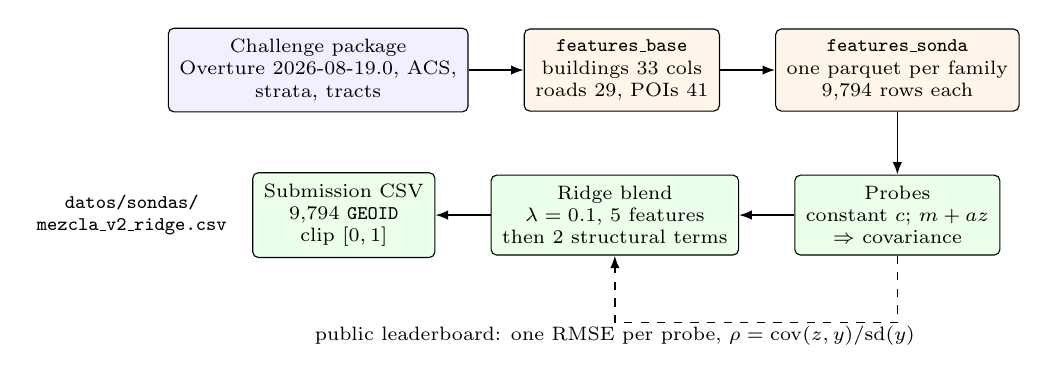
\begin{tikzpicture}[
  node distance=4mm and 7mm,
  box/.style={draw, rounded corners=2pt, align=center, font=\scriptsize,
              inner sep=4pt, minimum height=8mm, fill=black!3},
  data/.style={box, fill=blue!6},
  feat/.style={box, fill=orange!8},
  meth/.style={box, fill=green!8},
  ar/.style={-{Latex[length=1.6mm]}, semithick},
  ar2/.style={-{Latex[length=1.6mm]}, semithick, dashed}]

\node[data] (pkg) {Challenge package\\Overture 2026-08-19.0, ACS,\\strata, tracts};
\node[feat, right=of pkg] (base) {\texttt{features\_base}\\buildings 33 cols\\roads 29, POIs 41};
\node[feat, right=of base] (sonda) {\texttt{features\_sonda}\\one parquet per family\\9,794 rows each};
\node[meth, below=8mm of sonda] (probe) {Probes\\constant $c$; $m+a z$\\$\Rightarrow$ covariance};
\node[meth, left=of probe] (mix) {Ridge blend\\$\lambda=0.1$, 5 features\\then 2 structural terms};
\node[meth, left=of mix] (sub) {Submission CSV\\9,794 \texttt{GEOID}\\clip $[0,1]$};
\draw[ar] (pkg) -- (base);
\draw[ar] (base) -- (sonda);
\draw[ar] (sonda) -- (probe);
\draw[ar] (probe) -- (mix);
\draw[ar] (mix) -- (sub);
\draw[ar2] (probe.south) -- ++(0,-0.85) -|
  node[pos=0.55, below, font=\scriptsize, align=center]
  {public leaderboard: one RMSE per probe, $\rho=\mathrm{cov}(z,y)/\mathrm{sd}(y)$}
  (mix.south);

\node[font=\scriptsize, left=2mm of sub, align=center] {\texttt{datos/sondas/}\\\texttt{mezcla\_v2\_ridge.csv}};
\end{tikzpicture}
\caption{Architecture. The package produces two feature blocks; each candidate feature is
scored once as a leaderboard probe, which returns a covariance, not an accuracy; the blend
is a ridge combination of z-scored features plus the public mean.}
\label{fig:arch}
\end{figure}

Figure~\ref{fig:arch} is the whole method. Steps~2--4 of the pipeline (buildings, roads,
POIs) are the expensive ones: DuckDB over a \SI{5.8}{\giga\byte} package, with
\texttt{PRAGMA threads=2} and \texttt{SET memory\_limit='4GB'} fixed in the scripts.
Everything after
the features is seconds. Stage timings are in Section~\ref{sec:repro}.

\section{Two identities that make the leaderboard measure something}
\label{sec:identities}

\subsection{One constant submission measures the mean of the target}

For a constant prediction $f\equiv c$,
\begin{equation}
\R^2(c) = c^2 - 2c\,\mathbb{E}[y] + \mathbb{E}[y^2],
\end{equation}
so a constant submission leaves two unknowns and two constants solve them. The zero
submission scored \num{0.107246299}, hence $\mathbb{E}[y^2]=\num{0.011502}$. A constant
\num{0.05} scored \num{0.089560921}, hence
\[
\mathbb{E}[y] = \frac{0.0115018 + 0.0025 - 0.089560921^2}{0.1} = \num{0.059806},
\qquad \mathrm{sd}(y) = \sqrt{\mathbb{E}[y^2]-\mathbb{E}[y]^2} = \num{0.089022}.
\]
The optimal constant is the mean and its RMSE is the standard deviation: the floor to beat
is \num{0.089022}, not \num{0.107}. This costs one submission and no labels.

\subsection{A small-amplitude probe measures a covariance}

Take $m=\mathbb{E}[y]$ from the previous step and submit $f = m + a\,z$ with $z$ standardised
across all \num{9794} rows and $a=\num{0.02}$. Then
\begin{equation}
\R^2(f) = \mathrm{Var}(y) - 2a\,\mathrm{cov}(z,y) + a^2\,\mathbb{E}[z^2] + \big(m-\mathbb{E}_{\text{pub}}[y]\big)^2 ,
\end{equation}
and the level term vanishes. With $a=0.02$ the quadratic term is negligible, so
\[
\mathrm{cov}(z,y) = \frac{\mathrm{Var}(y) + a^2 - \R^2}{2a},
\qquad \rho = \frac{\mathrm{cov}(z,y)}{\mathrm{sd}(y)} .
\]
Each probe therefore returns a signed correlation between a feature and the hidden target.
The one approximation is $\mathbb{E}_{\text{pub}}[z^2]\approx 1$, taken from the full
\num{9794} rows rather than the public 30\%; its effect on $\R^2$ is of order $10^{-5}$ and on
$\rho$ about \num{0.003}. The six probes in Table~\ref{tab:probes} were spent this way, after the two constants fixed the level.

\begin{table}[htbp]
\centering
\small
\caption{Probes. Each row is one submission; $\rho$ is recovered from its public RMSE.}
\label{tab:probes}
\begin{tabular}{lrrr}
\toprule
Probe & Public RMSE & $\rho$ with $y$ & Verdict \\
\midrule
zero (control) & 0.107246299 & --- & gives $\mathbb{E}[y^2]$ \\
constant $0.05$ & 0.089560921 & --- & gives $\mathbb{E}[y]$, $\mathrm{sd}(y)$ \\
\Ftribal & 0.084907318 & $+0.313$ & strongest single signal \\
\Frural & 0.085765003 & $+0.272$ & kept \\
\Froute & 0.086122934 & $+0.255$ & kept \\
\Ftrans & 0.087594890 & $+0.183$ & kept \\
\Ffire & 0.088818198 & $+0.123$ & kept \\
\Fpoi & 0.091352474 & $-0.006$ & excluded: worse than the constant \\
\bottomrule
\end{tabular}
\end{table}

\section{Features and the blend}

Table~\ref{tab:features} lists the five features of the first blend. The transformation column is the
complete preprocessing, and there is no per-region fitting.

\begin{table}[htbp]
\centering
\caption{The five features of the first blend, their measured correlation with the hidden
score, their ridge coefficients at $\lambda=0.1$, the RMSE cost of dropping each one and, below,
each feature's source and transformation.}
\label{tab:features}
\footnotesize\setlength{\tabcolsep}{3pt}
\begin{tabular}{lrrrp{6.3cm}}
\toprule
Feature & $\rho$ with $y$ & $\beta$ ($\lambda=0.1$) & $\Delta$RMSE if dropped & Definition \\
\midrule
\texttt{r\_tribal\_any} & +0.313 & +0.0198 & +0.00264 & $1[$tract intersects a tribal area$]$, 874 tracts = 8.9\% \\
\texttt{g\_transport} & +0.183 & +0.0141 & +0.00147 & cand\_00 transport gap, $1.0$ when $km_{hw}=0$; $\rho=0.944$ with $1-km_{hw}/(km_{hw}+km_{tert}+km_{hw,ring25})$ \\
\texttt{rural} & +0.272 & +0.0125 & +0.00082 & $1[\texttt{pct\_urban}<0.5]$; NaN when \texttt{pct\_urban} is missing \\
\texttt{t\_route\_lowclass\_share} & +0.255 & +0.0113 & +0.00067 & share of road km on a numbered route in the lowest Overture road classes \\
\texttt{h\_fire\_missing\_risk} & +0.123 & +0.0078 & +0.00043 & fire-station coverage deficit, 0 = no deficit \\
\midrule
Intercept $m$ & --- & 0.059806 & --- & public mean of $y$ (constant-0.05 submission) \\
Predicted RMSE & --- & 0.08002 & --- & 5-feature blend, $\sqrt{\mathrm{Var}(y)}$ = 0.089022 \\
\bottomrule
\end{tabular}

\smallskip

\small
\begin{tabular}{p{5.4cm}p{4.6cm}p{3.9cm}}
\toprule
Feature & Source & Transformation \\
\midrule
\texttt{rural} & \texttt{components\_cand00}.\newline\texttt{pct\_urban} = \texttt{pop\_urban}/\texttt{pop\_total}\newline (package strata, 2020 census) & z-score; NaN $\to 0$ = mean \\
\texttt{g\_transport} & \texttt{components\_cand00}.\newline\texttt{g\_transport} (Overture roads) & z-score; no imputation, no winsor \\
\texttt{t\_route\_lowclass\_share} & \texttt{s01\_routes.parquet}\newline (Overture named routes) & winsorise p1/p99, then z-score (79\% zeros, kurtosis 48) \\
\texttt{h\_fire\_missing\_risk} & \texttt{s03\_fire\_ems.parquet}.\newline Overture POIs \texttt{fire\_department} and\newline \texttt{ambulance\_and\_ems\_services} vs population & z-score; no imputation, no winsor \\
\texttt{r\_tribal\_any} & \texttt{s07\_rurality.parquet}.\newline Package strata column \texttt{tribal\_any} & z-score on a 0/1 column \\
\bottomrule
\end{tabular}

\end{table}

The blend is
\begin{equation}
f_i = m + z_i^\top \beta, \qquad
\beta = (S + \lambda I)^{-1} \hat{c}, \qquad
\R^2 = \mathrm{Var}(y) - 2\beta^\top \hat{c} + \beta^\top S \beta,
\end{equation}
where $\hat{c}$ is the vector of covariances recovered by the probes, $S$ the sample
covariance matrix of the z-scored features over the \num{9794} rows and $\lambda=0.1$ a
fixed constant of the script (\path{procesos/sondas/sondas_v2.py}, function \texttt{fit}).
$\lambda$ shrinks the coefficients of correlated features (\Frural{} and \Ftribal{} overlap;
\Ftrans{} and \Froute{} both read the Overture road network); it was fixed before any blend
was scored, and Section~\ref{sec:alt} shows its effect is small.

Two details affect the coefficients. First, \Ftrans{} equals $1.0$ whenever a
tract has no named highway --- a construction artefact inherited from the earlier candidate,
discussed in Section~\ref{sec:edge}. Second, \Ftribal{} is a 0/1 column z-scored, so its
coefficient is per unit of a binary indicator, not per percent.

\section{Two structural terms: the final submission}
\label{sec:struct}

The published formula says the score is a mean over \emph{defined} components, and that the road
component is undefined where the reference has no primary or secondary road. Overture's \texttt{routes}
field carries the numbered network, so we estimate $\hat{T}_i$ as the kilometres of a tract's roads on a numbered interstate, US, state or state-secondary
route, in any road class (\path{procesos/sondas/s12_vias_red.py}), and flag the road component as likely
undefined when $\hat{T}_i\le\SI{0.25}{km}$. Table~\ref{tab:undef} compares that share with the published
share of tracts having at least one undefined component. These are different quantities, because the
published one counts all three components, but the closeness is why we kept the flag. $\hat{T}$ only
approximates the reference: the resulting Overture-to-$\hat{T}$ length ratios run from 1.17 to 1.96 by
region, against a published 0.71 to 1.59.

\begin{table}[htbp]
\centering
\small
\caption{Share of tracts with no numbered route in Overture, against the published share with at least
one undefined component. Eastern Washington has no published figure.}
\label{tab:undef}
\begin{tabular}{lrr}
\toprule
Region & No numbered route & Published \\
\midrule
\texttt{eastern-ok} & 25.7\% & 21\% \\
\texttt{northern-ca} & 41.3\% & 37\% \\
\texttt{south-central-tx} & 25.0\% & 28\% \\
\texttt{maricopa-az} & 58.9\% & 55\% \\
\texttt{eastern-wa} & 26.0\% & --- \\
\bottomrule
\end{tabular}
\end{table}

For facilities, each type's Overture count is fitted with a Poisson regression on rurality, log
population, log land area, log buildings and region, giving $\lambda_i$. If Overture holds a share $c$ of
the real facilities, what is missing is $M_i\sim\mathrm{Poisson}(\lambda_i(1-c)/c)$, independent of the
observed count $O_i$, and the expected gap is $\mathbb{E}[M_i/(O_i+M_i)]$ when $O_i+M_i>0$
(\path{procesos/sondas/s13_estructural.py}). We assumed $c=0.80$ for schools; it is not estimated,
and the leaderboard sets only the term's overall size.

We measured four candidates, each as submission 11 plus $0.02\,z$. Now
$\R^2(b+az)=\R^2(b)-2ac+a^2$, so a submission returns $c$, the covariance of $z$ with what the blend
still misses. The measurement error of $c$ is roughly $0.08/\sqrt{0.3\times9794}=\num{0.0015}$, an
approximation that treats the public rows as a random sample.

\begin{table}[htbp]
\centering
\small
\caption{The four last probes. A score above the no-effect value of 0.08268 means the step went the wrong
way, and that is information: the road flag has the strongest signal of the set, with a negative sign.}
\label{tab:probes2}
\begin{tabular}{lrrrl}
\toprule
Candidate (submission ID) & Public RMSE & $c$ & $c$/error & Decision \\
\midrule
\texttt{s\_road\_undefined} (NEhoA7Bd) & 0.08663476 & $-0.01673$ & $-11.3$ & kept, weight $-0.01522$ \\
\texttt{s\_poi\_schools} (yzRTSBH5) & 0.081699336 & $+0.00404$ & $+2.7$ & kept, weight $+0.00373$ \\
\texttt{s\_road\_gap\_condal} & 0.08200541 & $+0.00279$ & $+1.9$ & dropped \\
\texttt{b\_bldg\_deficit} (dQQyhb5r) & 0.083192057 & $-0.00211$ & $-1.4$ & dropped \\
\bottomrule
\end{tabular}
\end{table}

The road \emph{gap} estimate, the term we expected to matter most, added almost nothing: its joint weight
is 0.0001, because the five-feature blend already carries that signal through its rural, tribal and route
variables. Tracts with no numbered route have smaller scores than the blend predicted, which is consistent
with a component that cannot contribute a gap where it is undefined; the components themselves are not
observed. The final prediction, with $b_i$ the 5-feature blend, is
\begin{equation}
f_i = b_i - 0.01522\,z_i^{\text{no route}} + 0.00373\,z_i^{\text{schools}},
\end{equation}
clipped to $[0,1]$, with weights from the same ridge at $\lambda=0.1$. Predicted \num{0.07837}; returned
\textbf{\num{0.078391501}} (submission KDVKc3sY), a discrepancy of $+\num{0.00002}$.

\section{Relation to the organiser's three components}

The organiser's reference score is an unweighted mean of a road gap, a building gap and a POI
gap (itself a mean of a facilities half and an establishments half), with undefined
components dropped. The model relates to them as follows:

\begin{itemize}
\item roads: a \emph{within-Overture} statistic (\Froute) and a gap proxy (\Ftrans);
\item buildings: no term, because the building-deficit probe stayed within measurement error;
\item POIs: the expected school gap and the fire-station signal; the probe on total POIs (\Fpoi) measured no
signal and was dropped;
\item an estimate of where the road component is undefined, which the divisor of the published mean
makes relevant.
\end{itemize}

What survives is a set of correlates of the hidden score: rurality, tribal presence,
low-class route share, a transport-gap proxy, fire-station deficit, no numbered route, missing schools. The
largest coefficient is the tribal indicator.

\section{Edge cases}
\label{sec:edge}

Table~\ref{tab:edge} reports zero-population tracts, water-dominated tracts and tracts with no Overture data.
\textbf{No edge case has a branch of its own.} The global handling is a p1/p99 winsor on \Froute, z-scoring
with NaN filled by the feature mean (\texttt{features()} in \path{procesos/sondas/sondas_v2.py}) and a clip to
$[0,1]$ at the end that affects zero rows of the 5-feature blend. In the final submission the clip sets 59 rows to
0, all of them tracts with no numbered route. Table~\ref{tab:edge} reports the 5-feature blend.

\begin{table}[htbp]
\centering
\caption{Edge cases: counts, prediction levels relative to the global mean of \num{0.05981}, and
the treatment each one receives.}
\label{tab:edge}
\footnotesize\setlength{\tabcolsep}{3pt}
\begin{tabular}{lrrrrrrr}
\toprule
Case & $n$ & \% of tracts & Mean pred. & Min & Max & Ratio & \texttt{pct\_urban} NaN \\
\midrule
pop0 & 27 & 0.28 & 0.06048 & 0.02814 & 0.09500 & 1.01$\times$ & 27 \\
water50 & 43 & 0.44 & 0.06194 & 0.01821 & 0.17223 & 1.04$\times$ & 2 \\
water90 & 3 & 0.03 & 0.08713 & 0.07139 & 0.09500 & 1.46$\times$ & 2 \\
nobldg & 2 & 0.02 & 0.09500 & 0.09500 & 0.09500 & 1.59$\times$ & 2 \\
noroad & 1 & 0.01 & 0.09500 & 0.09500 & 0.09500 & 1.59$\times$ & 1 \\
nopoi & 2 & 0.02 & 0.09500 & 0.09500 & 0.09500 & 1.59$\times$ & 2 \\
nohighway & 137 & 1.40 & 0.11807 & 0.08894 & 0.21470 & 1.97$\times$ & 7 \\
\midrule
All tracts & 9794 & 100.00 & 0.05981 & 0.01539 & 0.26101 & 1.00$\times$ & 27 \\
\bottomrule
\end{tabular}

\par\smallskip\footnotesize
Ratio = mean prediction inside the case / global mean (0.05981). Predictions are the submitted 5-feature blend (\texttt{mezcla\_v2\_ridge.csv}); 0 of 9{,}794 rows hit the $[0,1]$ clip.
\begin{tabular}{lrrrrrr}
\toprule
Case & eastern-ok & eastern-wa & maricopa-az & northern-ca & south-central-tx & All \\
\midrule
\multicolumn{7}{l}{\emph{Cells: $n$ / mean prediction}} \\
\midrule
pop0 & 1 / 0.0417 & 1 / 0.0538 & 11 / 0.0626 & 0 / --- & 14 / 0.0606 & 27 / 0.0605 \\
water50 & 1 / 0.0525 & 0 / --- & 0 / --- & 2 / 0.0207 & 40 / 0.0642 & 43 / 0.0619 \\
water90 & 0 / --- & 0 / --- & 0 / --- & 0 / --- & 3 / 0.0871 & 3 / 0.0871 \\
nobldg & 0 / --- & 0 / --- & 0 / --- & 0 / --- & 2 / 0.0950 & 2 / 0.0950 \\
noroad & 0 / --- & 0 / --- & 0 / --- & 0 / --- & 1 / 0.0950 & 1 / 0.0950 \\
nopoi & 0 / --- & 0 / --- & 0 / --- & 0 / --- & 2 / 0.0950 & 2 / 0.0950 \\
nohighway & 28 / 0.1550 & 5 / 0.1160 & 33 / 0.1077 & 7 / 0.1184 & 64 / 0.1074 & 137 / 0.1181 \\
\midrule
Region mean pred. & 0.1134 & 0.0664 & 0.0521 & 0.0580 & 0.0509 & 0.0598 \\
Region $n$ & 1192 & 415 & 1593 & 591 & 6003 & 9794 \\
\bottomrule
\end{tabular}

\smallskip

\begin{tabular}{p{1.7cm}p{11.4cm}}
\toprule
Case & Treatment in the pipeline \\
\midrule
pop0 & no mask, no imputation; same formula. 27/27 lack \texttt{pct\_urban}, so \texttt{rural} is undefined and the z-fill sets it to its mean \\
water50 & no mask. Both water-only tracts (ALAND $=0$) have $km_{hw}=0$, so \texttt{g\_transport} takes its maximum value 1.0 \\
water90 & same as above; the third tract (0.93 water) has 3{,}005 residents and 3{,}093 buildings \\
nobldg & no mask in the blend. In the cand\_00 block a building-less tract gets the maximum gap, not a missing value \\
noroad & no mask; \texttt{km\_highway}$=0$ gives \texttt{g\_transport}$=1.0$ (maximum gap), the opposite of a fully mapped tract \\
nopoi & no mask in the blend; \texttt{components.py} returns 0 only for a zero expectation denominator (not in the final blend) \\
nohighway & no mask; \texttt{g\_transport}$=1.0$ for all 137 by construction of the cand\_00 column \\
\bottomrule
\end{tabular}
\end{table}

The structural terms lower the edge cases without treating them specially: mean predictions in the
final submission are \num{0.04910} for zero-population tracts (27), \num{0.09985} for tracts with no named
highway (137) and \num{0.06645} for the two water-only tracts. Tracts with no numbered route (\num{3096})
move from \num{0.05204} to \num{0.02973}, and the rest (\num{6698}) from \num{0.06340} to \num{0.07373}.

The 5-feature blend has two artefacts.

\begin{enumerate}
\item \textbf{137 tracts with no named highway receive \Ftrans$\,=1.0$}, the maximum possible
gap, because that column is set to $1.0$ exactly when $km_{highway}=0$
(\texttt{components()} in \path{procesos/step_09_ensemble/script.py}). Their
mean prediction is \num{0.11807}, 1.97$\times$ the global mean, and 28 of them are in
Eastern Oklahoma. Some of them are tracts where a highway genuinely
is missing from Overture; others are tracts where the highway exists but is unnamed or
classified differently, and for those the model asserts a maximum gap that no data supports.
\item \textbf{The two water-only tracts (ALAND $=0$, both with zero population) receive
\num{0.09500}}, 1.59$\times$ the global mean and the value shared by every degenerate case: no
highway, no building, no POI, so every term that can saturate does. Other no-highway tracts reach
\num{0.21470}. They are inside the 137 above, not an extra case. The
third tract of the water-dominated bucket is 0.93 water but has 3{,}005 residents and
3{,}093 buildings, and sits at \num{0.07139}.
\end{enumerate}

\Ftrans{} stays because those are 1.4\% of tracts and its incremental contribution to the blend is
\num{0.00147}. Masking or shrinking the 137 was not tested: each test costs a submission, at five per day.

\section{Alternative weightings and their cost}
\label{sec:alt}

\begin{table}[htbp]
\centering
\caption{Alternative weightings. Mix4, the 5-feature blend and its $s=0.85$ shrink were
submitted; the others are predictions from the validated covariance identity.}
\label{tab:alt}
\footnotesize\setlength{\tabcolsep}{3pt}
\begin{tabular}{lcrrrrr}
\toprule
Blend & $\lambda$ & Shrink $s$ & Pred. RMSE & $\Delta$ vs mix4 & LB RMSE & corr with 5-feature blend \\
\midrule
mix4 (submission 9) & 0.1 & 1.00 & 0.08265 & --- & 0.082736583 & 0.8518 \\
\texttt{mezcla\_v2\_ridge} (submission 11) & 0.1 & 1.00 & 0.08002 & -0.00264 & 0.080228114 & 1.0000 \\
\texttt{mezcla\_v3\_lam03} & 0.3 & 1.00 & 0.08027$^{\dagger}$ & -0.00238 & --- & 0.9997 \\
\texttt{mezcla\_v3\_shrink85} (submission 12) & 0.1 & 0.85 & 0.08023 & -0.00243 & 0.080525733 & 1.0000 \\
\texttt{mezcla\_v3\_sin\_fire} & 0.1 & 1.00 & 0.08045$^{\dagger}$ & -0.00220 & --- & 0.9773 \\
\bottomrule
\end{tabular}

\par\smallskip\footnotesize $^{\dagger}$Predicted, not submitted: no leaderboard RMSE exists. Predicted RMSE uses the measured covariance identity $RMSE^2=\mathrm{Var}(y)-2\beta^{\top}c+\beta^{\top}S\beta$, with $S$ the sample covariance of the z-scored features and $c$ the covariance with $y$ implied by each probe's public score; the identity was validated on submission 9 ($+0.000087$). Predictions here chain from the predicted RMSE of the blend, not its real score. Correlation is Pearson over the 9{,}794 predictions against the 5-feature blend. Shrinking by $s$ gives $RMSE^2=\mathrm{Var}(y)-(2s-s^2)(\mathrm{Var}(y)-RMSE_0^2)$. $\Delta$ is against the submitted 4-feature blend (predicted 0.082654).
\end{table}

Three alternatives to the blend were built. Two were predicted but never submitted, because
the submission budget was five per day and those slots went to measurements: stronger
regularisation ($\lambda=0.3$) is predicted to cost \num{0.00025} against the 5-feature blend and
dropping the weakest feature (\Ffire) \num{0.00043}. The third, shrinking the whole blend by $s=0.85$, was submitted
as a hedge against the private split moving (submission 12) and returned
\num{0.080525733}, \num{0.000298} worse than the unshrunk blend. Computed from the blend's real
score, the identity predicts \num{0.080558} for that shrink, a discrepancy of
$-\num{0.00003}$: a third validation. The same arithmetic gives an optimal scale of 1.06 on
the public split, so the unshrunk blend is about the right size. We keep it as the primary
submission because a shrink factor chosen after seeing the public score is a second free
parameter fitted to 30\% of the data.

For the two structural terms we compared variants by predicted RMSE, without submitting them: the road
flag alone \num{0.07848}; adding the school term \num{0.07837}, the choice; adding all four \num{0.07836};
the same at $\lambda=0$ \num{0.07835}; shrinking the three-term version to 0.9 \num{0.07841}. These
differences are smaller than the measurement error, so we kept only terms above two errors.

\section{Results}

\begin{table}[htbp]
\centering
\small
\caption{Submitted sequence. $\Delta$ is against the optimal constant (\num{0.089022}).}
\begin{tabular}{llrr}
\toprule
Step & What it is & Public RMSE & $\Delta$ vs constant \\
\midrule
1 & zero & 0.107246299 & $+0.018224$ \\
3 & constant 0.05 (measures $\mathbb{E}[y]$) & 0.089560921 & $+0.000539$ \\
9 & blend of 4 features & \textbf{0.082736583} & $-0.006285$ \\
11 & blend of 5 features (submitted) & \textbf{0.080228114} & $-0.008794$ \\
12 & the same blend shrunk by $s=0.85$ & 0.080525733 & $-0.008497$ \\
13--16 & four probes on top of the blend (Table~\ref{tab:probes2}) & see table & --- \\
17 & final: blend + road flag + school term & \textbf{0.078391501} & $-0.010631$ \\
\bottomrule
\end{tabular}
\end{table}

The 4-feature blend was predicted at \num{0.08265} and returned \num{0.082736583}: a
discrepancy of $+\num{0.000087}$, 5.7 times below the \num{0.0005} tolerance fixed before
uploading. That is the validation of the only approximate quantity in the method
($\mathbb{E}_{\text{pub}}[z^2]\approx1$). The 5-feature blend was then predicted at
\num{0.08002} and returned \num{0.080228114}, $+\num{0.000208}$ --- still inside the
tolerance. Adding a fifth feature bought \num{0.0025}, and each individual probe's contribution (\num{0.0004} to \num{0.0026})
is small taken alone, which is why the blend, not the probes, is the deliverable.

The final blend's $R^2\approx0.22$ means it explains about a fifth of the variance of the target.

\section{Reproducibility}
\label{sec:repro}

The pipeline is deterministic: there is no sampling, no stochastic optimiser and no train/test
split, so no seed exists to fix. Every script resolves the repository root from
\texttt{\_\_file\_\_}, reads the challenge package and writes to \texttt{datos/}.

\begin{verbatim}
bash procesos/run_all.sh        # steps 1-9, in order
\end{verbatim}

A clean clone was built on 30 October 2026, with the challenge package supplied separately, and the
chain re-run:

\begin{table}[htbp]
\centering
\small
\caption{Clean-clone reproduction. Wall-clock times.}
\begin{tabular}{lrr}
\toprule
Stage & Script & Time \\
\midrule
buildings & \texttt{step\_02\_buildings/script.py} & \SI{835}{s} \\
roads & \texttt{step\_03\_roads/script.py} & \SI{2070}{s} \\
POIs & \texttt{step\_04\_pois/script.py} & \SI{72}{s} \\
candidate ensemble & \texttt{step\_09\_ensemble/script.py} & \SI{2}{s} \\
probe features & \texttt{probes\_s01\_s10/sNN\_*.py} & \SI{376}{s} \\
probe build & \texttt{sondas/sondas\_v2.py build} & \SI{3}{s} \\
blend & \texttt{sondas/sondas\_v2.py read} & \SI{2}{s} \\
\midrule
total & & \SI{56}{min} \\
\bottomrule
\end{tabular}
\end{table}

Agreement with the repository's own artefacts: \texttt{mezcla\_v2\_ridge.csv} reproduced with
an \emph{identical} SHA-256; \texttt{features\_buildings.parquet} differs by at most
\num{6.3e-09} on \texttt{bldg\_area\_total\_m2} and \num{6.7e-16} on \texttt{confidence\_mean};
\texttt{features\_roads.parquet} and \texttt{components\_cand00.parquet} are bit-identical;
\texttt{features\_pois.parquet} differs by \num{3.0e-15} on \texttt{confidence\_mean}. The two
probe parquets that differ by hash differ only in row order.

The structural step was re-run from the Overture layers on 31 October 2026
(\path{s12_vias_red.py}, \path{s13_estructural.py}, \path{secuencial.py sondas}): the final CSV and the four
probe CSVs reproduced with identical SHA-256. The final CSV is
\path{datos/sondas/mezcla_v4_estructural.csv}. The timings above predate that step, which takes about
four minutes.

One warning for anyone re-running: \texttt{sondas\_v2.py read} \emph{overwrites}
\texttt{mezcla\_v2\_ridge.csv}. It is the last step for that reason.

\section{Limitations}

\begin{enumerate}
\item \textbf{The weights come from probing the public leaderboard.} Every covariance in
Table~\ref{tab:probes} is one public RMSE on 30\% of the test set. The identity has been
validated four times (4 features, 5 features, shrunk blend, final; $|\Delta|\le\num{0.00021}$), but a covariance measured on
30\% of the tracts is not the covariance of the private 70\%. If the public split is not
representative --- by region, by rural share, or by the mix of tribal tracts --- the blend's
coefficients are biased in exactly the direction of that unrepresentativeness, and we have no
way to detect it without the private labels.
\item The floor \num{0.089022} and the mean \num{0.059806} are properties of the \emph{public}
split. They are used as constants in the blend, so a private mean that differs shifts every
prediction.
\item The blend extrapolates the covariance identity linearly; the second-order term is
discarded. At $a=0.02$ it is negligible per probe, but with five features it is no longer
strictly negligible.
\item The road flag is a proxy: $\hat{T}$ matches the published undefined shares to within five points but
misses its length ratios, the school coverage $c=0.80$ is assumed, and no term was checked tract by tract.
\item Nothing here validates against the organiser's components. A tract can score well and
still be wrong about which component is missing.
\end{enumerate}

\end{document}
